\documentclass[11pt]{article}
%\documentclass[preprint, 10pt]{elsarticle}

% PACKAGES
\usepackage{graphicx, amsmath, amssymb, amsfonts, mathtools, mathrsfs, color}
\usepackage{comment, enumerate, tabularx}
\usepackage{natbib, hyperref, url}
\usepackage[margin=1in]{geometry}
%\usepackage[justification=RaggedRight]{caption}

%----------------------------------------------------------------------------%
%% LATEX DEFINITIONS
%----------------------------------------------------------------------------%
% Basic editing
\newcommand{\tocite}{{\color{blue}(to cite)}}
\newcommand{\vsp}[1]{\vspace{#1 pc} \noindent}
\newcommand{\np}{\newpage \noindent}
% Derivatives
\newcommand{\pd}[2]    { \frac{\partial #1} {\partial #2} }
\newcommand{\ppd}[2]  { \frac{\partial^2 #1}{{\partial #2}^2} }
\newcommand{\pdi}[2] { {\partial_#2} #1 }
\newcommand{\td}[2] { \frac{d #1} { d #2 } }
\newcommand{\grad}{\nabla}
\newcommand {\Lap} {\grad^2}
% Vectors and operators
\newcommand{\bvec}[1]{\ensuremath{\boldsymbol{#1}}}
\newcommand{\abs}[1]{\left| #1 \right|}
\newcommand{\norm}[1]{\left\| #1 \right\|}
\newcommand{\mean}[1]{\left< #1 \right>}
\newcommand{\eps}{\varepsilon}
\newcommand{\dx}{\, dx}
% Basic physical parameters and scales
\newcommand{\freqp}{f_p}
\newcommand{\etastd}{\eta_{\text std}}
% Parameters that change crossing the ADC
\newcommand{\depth}{d}
\newcommand{\dup}{\depth_{-}}
\newcommand{\ddn}{\depth_{+}}
\newcommand{\dupdn}{\depth_{\pm}}
\newcommand{\lam}{\lambda}
\newcommand{\lamup}{\lam_{-}}
\newcommand{\lamdn}{\lam_{+}}
\newcommand{\lamupdn}{\lam_{\pm}}
\newcommand{\lamfac}{N}
\newcommand{\drat}{\mathcal{D}}
\newcommand{\dratdn}{\drat_+}
\newcommand{\dratupdn}{\drat_{\pm}}
% Statistical quantities
\newcommand{\En}{\mathcal{E}}
\newcommand{\Mo}{\mathcal{M}}
\newcommand{\skw}{\text{skew}}
\newcommand{\skwdn}{\skw_+}
\newcommand{\var}{\text{var}}
\newcommand{\varup}{\var_-}
\newcommand{\vardn}{\var_+}
% Dimensionless parameters
\newcommand{\ampscale}{\mathcal{A}}
\newcommand{\lengthscale}{\mathcal{L}}
\newcommand{\timescale}{\mathcal{T}}
\newcommand{\epsup}{\eps_0}
\newcommand{\delup}{\delta_0}
% Hamiltonian and Gibbs stuff
\newcommand{\uhat}{\hat{u}}
\newcommand{\Ham}{\mathcal{H}}
\newcommand{\Hthree}{\Ham_{3}}
\newcommand{\Htwo}{\Ham_{2}}
\newcommand{\Hup}{\Ham^{-}}
\newcommand{\Hdn}{\Ham^{+}}
\newcommand{\Hupdn}{\Ham^{\pm}}
\newcommand{\Gibbs}{\mathcal{G}}
\newcommand{\Gup}{\Gibbs^{-}}
\newcommand{\Gdn}{\Gibbs^{+}}
\newcommand{\Gupdn}{\Gibbs^{\pm}}
\newcommand{\thup}{\theta^{-}}
\newcommand{\thdn}{\theta^{+}}
\newcommand{\thupdn}{\theta^{\pm}}
\newcommand{\meanup}[1]{\mean{#1}_{-}}
\newcommand{\meandn}[1]{\mean{#1}_{+}}
\newcommand{\meanupdn}[1]{\mean{#1}_{\pm}}


% Experiments
\newcommand{\omavg}{\omega_0}
\newcommand{\omsig}{\sigma_{\omega}}
%----------------------------------------------------------------------------%

%----------------------------------------------%
%% TITLE
%----------------------------------------------%
\begin{document}
%Deterministic and statistical truncated KdV models for anomalous waves induced by abrupt depth change
\title{The truncated KdV framework for modeling anomalous waves induced by abrupt depth changes}

\author{
C.~Tyler Bolles\thanks{University of Michigan},
Andrew J.~Majda\thanks{Courant Institute of Mathematical Sciences}, 
M.~N.~J.~Moore\thanks{Florida State University}, 
Di Qi\thanks{Courant Institute of Mathematical Sciences} }
\maketitle

%----------------------------------------------------------%
% Intro
%----------------------------------------------------------%
\section{Introduction}


Introduce waves. \\
Introduce papers: PRF, PNAS, and J Stat Phys. \\

The purpose of this manuscript is to:
\begin{itemize}
\item Provide a more comprehensive treatment of the experiments and theory in combination. In particular, we make new comparisons between theory and experiments, which further confirm the predictive power of the theoretical framework.
\item Provide more thorough treatment of the link between physical system parameters and model parameters. This will elucidate the connection between theory and experiments. In particular, we flesh out details of non-dimensionalization, which were only briefly discussed in \cite{majda2019statistical} for the sake of brevity.
\item Provide additional experimental measurements not presented in \cite{bolles2019anomalous}. For example, statistics on surface slope and autocorrelation.
\end{itemize}

%----------------------------------------------------------%
% Experiments
%----------------------------------------------------------%
\section{The experiments}

	As discussed in \cite{bolles2019anomalous}, the experiments consist of a long, narrow wave tank (6 m long x 20 cm wide x 30 cm high), with waves generated by plexiglass paddle at one end. The waves propagate through the tank and, roughly midway through, pass over an abrupt depth change (ADC), which is created by a plexiglass step. The waves continue to propagate through the shallower depth until reaching the far end of the tank, at which point their energy is dissipated by a horse-hair dampener. Since the dampener minimizes the backscatter, the waves in this experiment propagate primarily in one direction, from left to right in Fig.~\ref{fig1}. 

The pivoting motion of the paddle is driven by a 5-phase stepper motor. To generate a randomized incoming wave field, the paddle angle $\phi$ is specified by a precomputed psuedo-random signal
\begin{align}
\label{PaddleAngle}
& \phi(t) = \phi_0 + \Delta \phi \sum_{n=1}^N a_n \cos(\omega_n t+\delta_n) \, , \\
\label{anEq}
& a_n = \sqrt{\frac{2 \Delta \omega}{\pi^{1/2} \omsig}} \, 
\exp \left( -\frac{(\omega_n - \omavg)^2}{2 \omsig^2} \right) \, ,
\end{align}
(Literal copy and paste) Here, the angular frequencies are evenly spaced $\omega_n = n  \Delta \omega$ with step size $ \Delta \omega = (\omavg+4 \omsig)/N$, where $\omavg$ and $\omsig$ represent the mean and the bandwidth of $\omega$ respectively. We set $\omavg = \omsig = 12.5$ rad/s, corresponding to a peak forcing frequency of 2 Hz and bandwidth of 2 Hz. Importantly, the phases $\delta_n$ are uniformly distributed random variables. We fix $N = 3000$, which sets a fundamental period of $T = 300$ seconds.
	
 % Figure 1
%^^^^^^^^^^^^^^^^^^^^^^^^^^^^^^%
\begin{figure}%[!ht]
\begin{center}
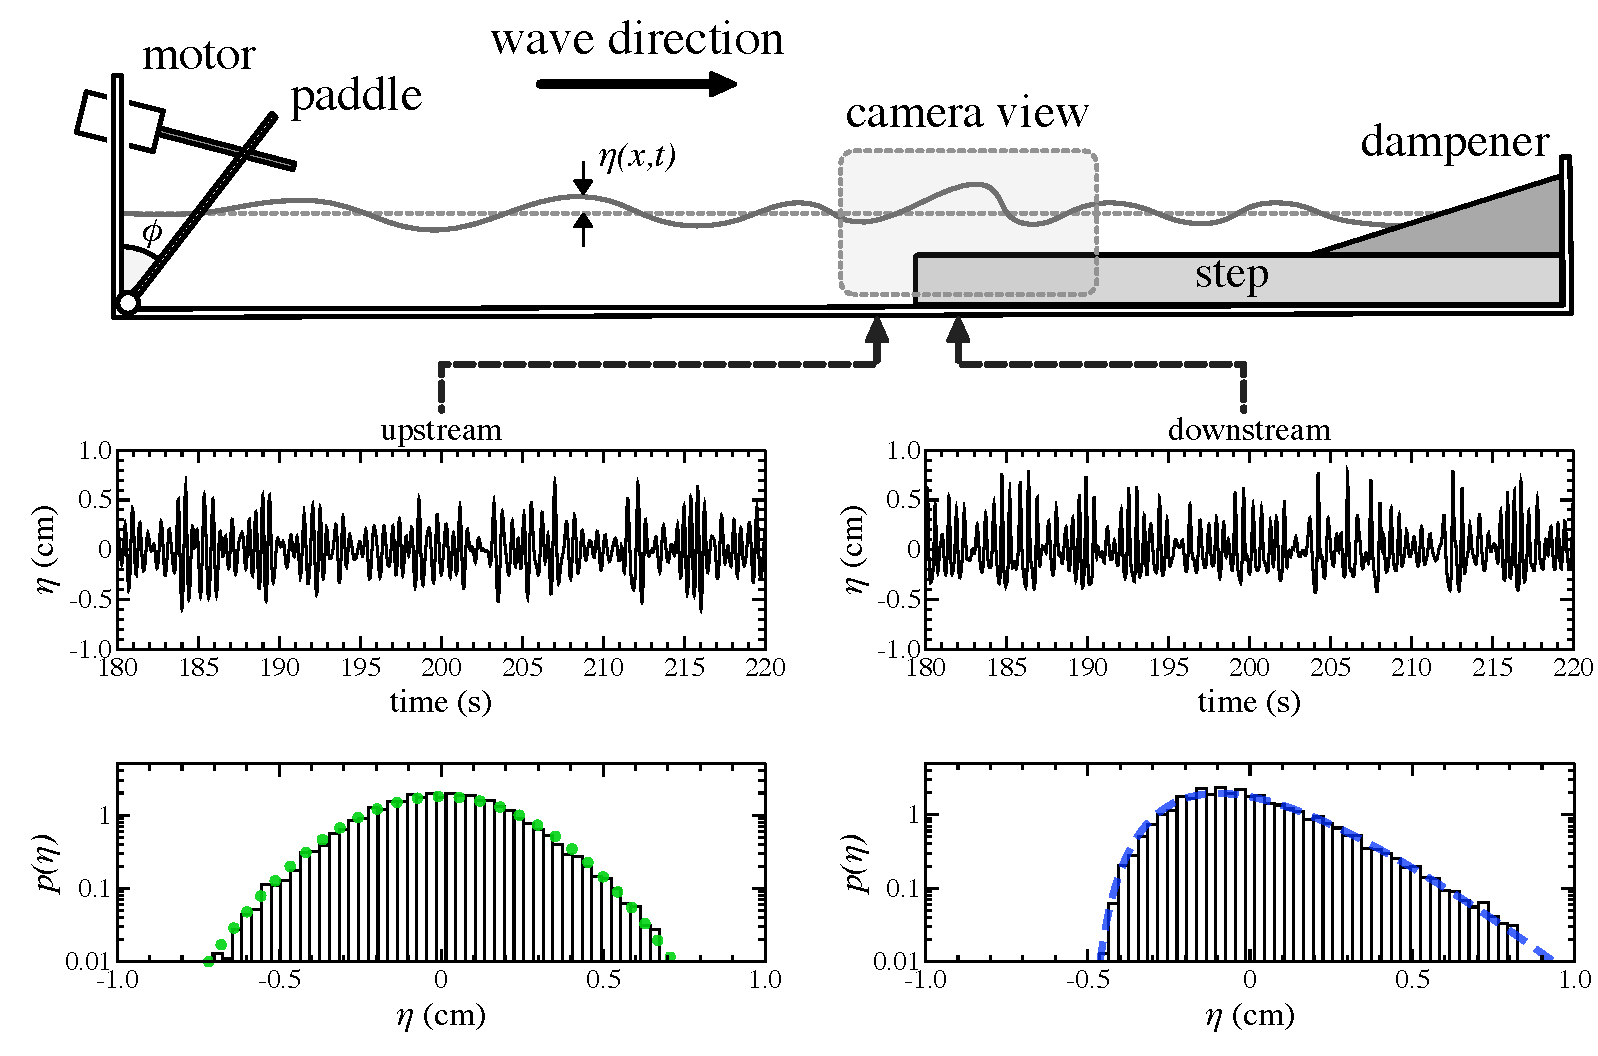
\includegraphics[width = 0.85 \linewidth]{Figs/fig1.pdf}
\caption{
(a) Experimental schematic. Reproduced from \cite{bolles2019anomalous}
}
%(b)--(c) Surface displacement measured at a representative upstream and downstream location. (d)--(e) Corresponding histograms.
\label{fig1}
\end{center}
\end{figure}
 %^^^^^^^^^^^^^^^^^^^^^^^^^^^^^^%

	The free surface is illuminated by light-emitting diodes running along the bottom of the tank and then imaged from the sideview with a Nikon D3300 at 60 frames per second. The illumination technique coupled with high pixel count of the camera allows surface displacements to be resolved with a accuracy better than 1/3 millimeter. Representative free surface measurements are shown in Figs.~\ref{fig2}(a)--(b) at a position upstream and downstream of the ADC. The corresponding histograms are shown in Figs.~\ref{fig2}(c)--(d).


 % Figure 2
%^^^^^^^^^^^^^^^^^^^^^^^^^^^^^^%
\begin{figure}%[!ht]
\begin{center}
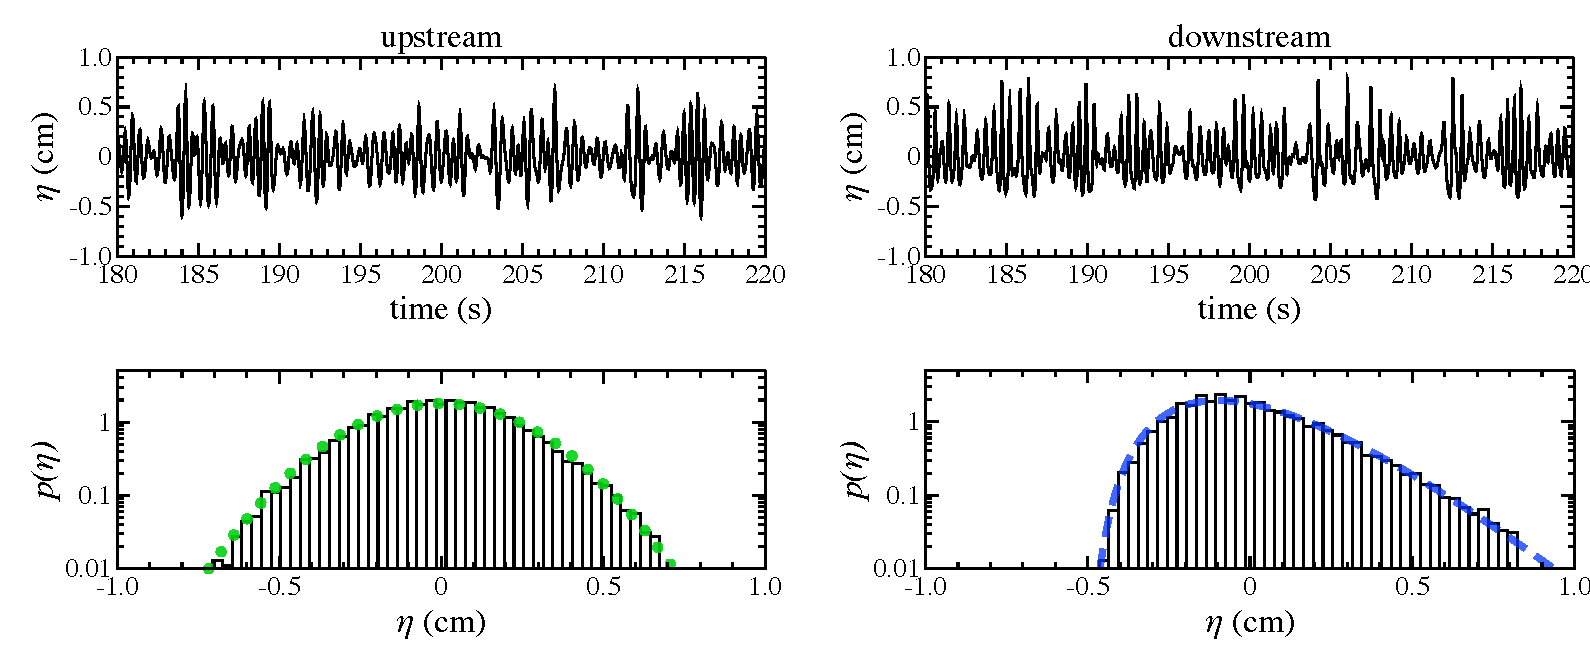
\includegraphics[width = 0.85 \linewidth]{Figs/fig2.pdf}
\caption{
(a)--(b) Surface displacement measured at a representative upstream and downstream location. (c)--(d) Corresponding histograms. Reproduced from \cite{bolles2019anomalous}
}
\label{fig2}
\end{center}
\end{figure}
 %^^^^^^^^^^^^^^^^^^^^^^^^^^^^^^%
 % Data from column 5 in MasterTimeSeries, Delta theta = 1.38 degrees, which is in between runs 5 and 6.
 
  % Figure 3
%^^^^^^^^^^^^^^^^^^^^^^^^^^^^^^%
\begin{figure}%[!ht]
\begin{center}
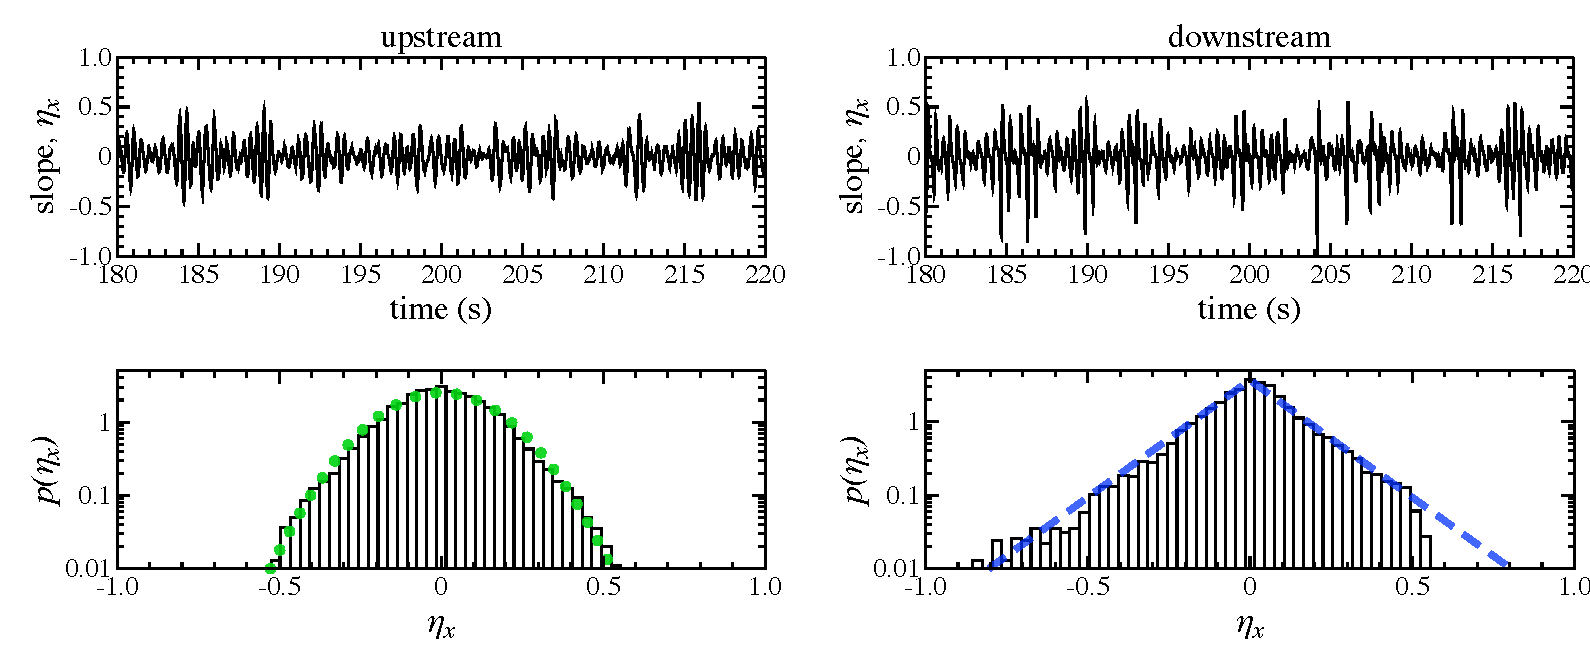
\includegraphics[width = 0.85 \linewidth]{Figs/fig3.pdf}
\caption{
(b)--(c) Surface slope measured at a representative upstream and downstream location. (d)--(e) Corresponding histograms. NEW PLOT.
}
\label{fig3}
\end{center}
\end{figure}
 %^^^^^^^^^^^^^^^^^^^^^^^^^^^^^^%
 
% Figure 4
%^^^^^^^^^^^^^^^^^^^^^^^^^^^^^^%
\begin{figure}%[!ht]
\begin{center}
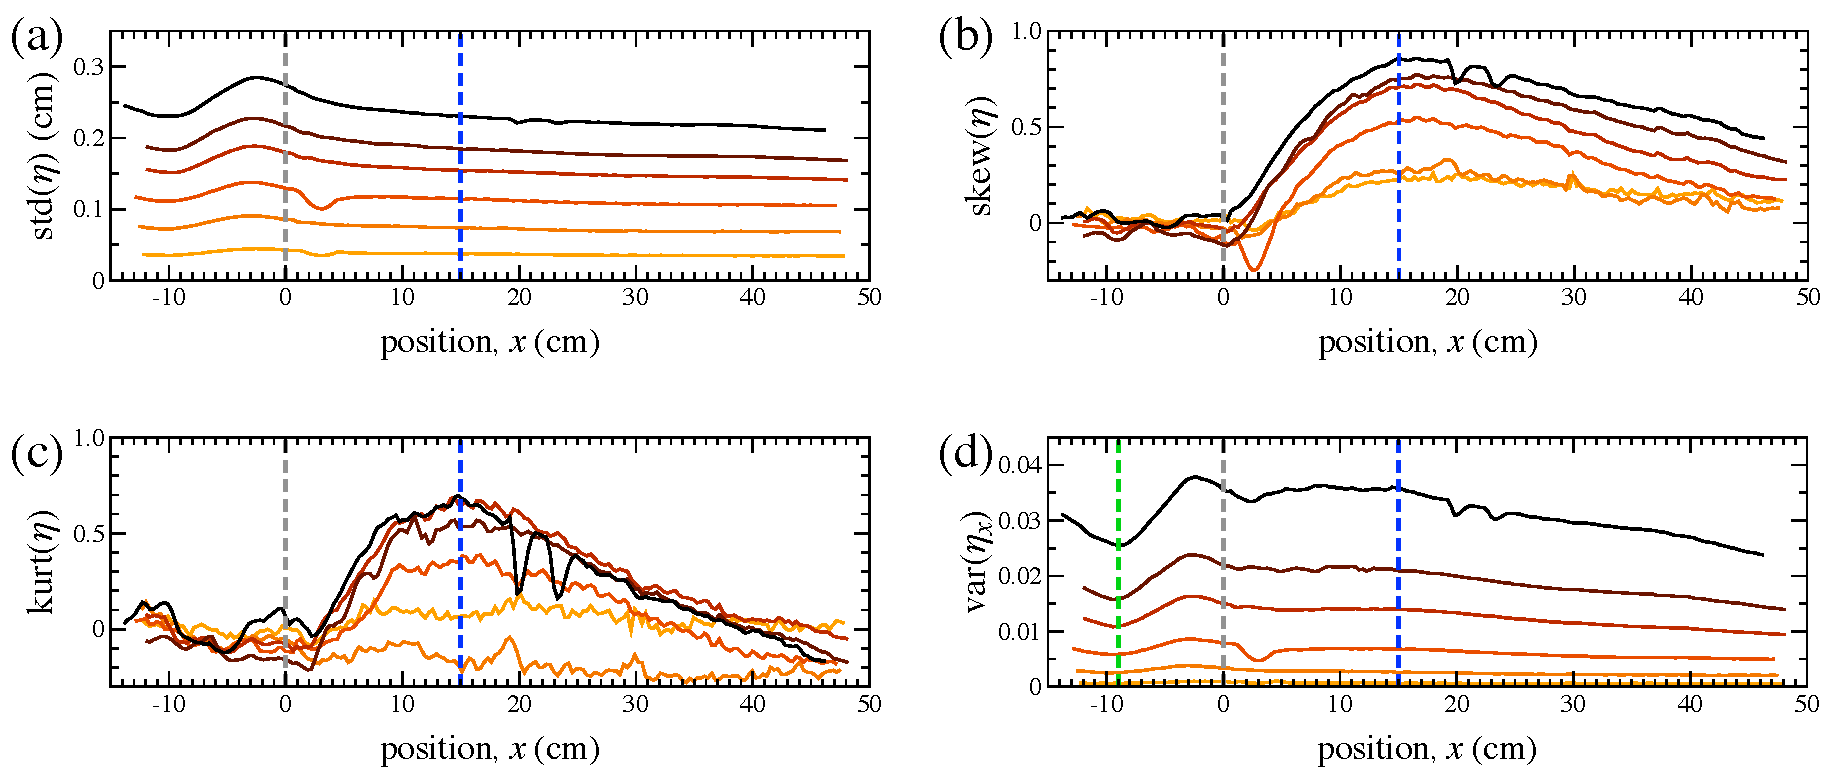
\includegraphics[width = 0.85 \linewidth]{Figs/fig4.pdf}
\caption{
Spatial statistics from the experiments.
}
\label{fig4}
\end{center}
\end{figure}
 %^^^^^^^^^^^^^^^^^^^^^^^^^^^^^^%
 
%----------------------------------------------------------%
% Theory
%----------------------------------------------------------%
\section{The truncated KdV framework}

%----------------------------------------------------------------------------%
% KdV
%----------------------------------------------------------------------------%
\subsection{The Korteweg–de Vries equation with variable depth}
Consider waves propagating unidirectionally in shallow water. Consider the surface displacement $\eta(x,t)$ and the reference frame moving with the local wave speed $\xi = x - ct$, where $c = \sqrt{g \depth}$ is the wave speed, $g$ gravity, and $\depth$ the local depth.
To first-correction in small amplitude, surface displacements are governed by the Korteweg–de Vries equation (KdV), which in dimensional form is given by \cite{whitham2011linear}
\begin{equation}
\label{KdV}
\eta_t + \frac{3 c}{2 \depth} \eta \eta_{\xi} + \frac{c \depth^2}{6} \eta_{\xi \xi \xi} = 0
\end{equation}
% This dimensional form is given by Whitham on p. 461, Eq. 13.98. I first got it from the Wolfram KdV, which gives the same equation.

We will primarily consider the case in which waves originate from a region of constant depth, encounter an abrupt depth change, and then continue in another region of constant depth. Thus, depth will be piecewise constant
\begin{align}
\depth = 
\begin{cases}
\dup \quad \mbox{if } x<0 \\
\ddn \quad \mbox{if } x>0
\end{cases}
\end{align}
Most often, we will consider waves moving into shallower depth, so that $\dup > \ddn$. 

The incoming waves are randomized and generated with a peak forcing frequency of $\freqp$, which gives rise to the following quantities
\begin{align}
&c = \sqrt{g \depth}
&&\mbox{\em local wave speed} \\
&\lam = c/\freqp = \sqrt{g \depth} / \freqp
&&\mbox{\em local peak wave length} \\
&\etastd = \mean{\eta^2}^{1/2} 
&&\mbox{\em surface displacement standard deviation} \\
\end{align}
where $\mean{\cdot}$ indicates the mean of a quantity. 
Note that the characteristic wave speed $c = c_{\pm}$ and wavelength $\lam = \lamupdn$ each take different values upstream and downstream of the ADC. We remark that experimental measurements indicate that $\etastd = \mean{\eta^2}^{1/2}$ is nearly the same on both values of the ADC. Hence, we will not distinguish between upstream and downstream values of $\etastd$.

%----------------------------------------------------------------------------%
% Nondimensionalization
%----------------------------------------------------------------------------%
\subsection{Nondimensionalization of variable-depth KdV}

In this section, the variable-depth KdV equation \eqref{KdV} will be recast into a dimensionless form chosen for convenience in working with the Hamiltonian/statistical-mechanics framework introduced in \cite{majda2019statistical}. Since the choice of how to normalize is not unique, it is instructive to first introduce a generic normalization to facilitate comparison with other choices. To this end, consider characteristic scales, $\ampscale, \lengthscale, \timescale$ for the wave amplitude, longitudinal length, and time respectively, which can remain unspecified for the moment. We introduce the dimensionless variables
\begin{align}
&u = \eta / \ampscale
&&\mbox{\em dimensionless surface displacement} \\
&\tilde{x} = \xi / \lengthscale
&&\mbox{\em dimensionless position (in moving frame)} \\
&\tilde{t} = t / \timescale
&&\mbox{\em dimensionless time}
\end{align}
Recasting \eqref{KdV} in terms of these variables and dropping the tildes for simplicity, gives the general dimensionless KdV equation:
\begin{equation}
u_t + \frac{3}{2} \left( \frac{c \timescale \ampscale}{\lengthscale \depth} \right) u u_x 
+ \frac{1}{6} \left( \frac{c \timescale \depth^2}{\lengthscale^3} \right) u_{xxx} = 0
\end{equation}

Now, the scales $\ampscale, \lengthscale, \timescale$ can be chosen for ease in working with a particular framework. In particular, we choose the following scales,
\begin{align}
\ampscale = \pi^{1/2} \, \etastd \, , \qquad
\lengthscale = \frac{\lamfac \lam}{\pi} \, , \qquad
\timescale = \frac{\lamfac \lam}{\freqp \depth}
\end{align}
where $\lamfac$ is an integer to be chosen later. 
The explanation for these choices is as follows. First, we have chosen the characteristic amplitude, $\ampscale$, above to normalize the energy of the state-variable $u$ to unity, as will be demonstrated in Section \ref{tKdVSec}. Second, regarding the choice of $\lengthscale$, recall that $\lam$ is the characteristic wavelength that corresponds to the peak forcing frequency $\freqp$ in the experiments. If only integer multiples of $\freqp$ were imposed (e.g.~lower frequencies were not present), then the forcing would produce waves that are periodic over the physical interval $\xi \in [-\lam,\lam]$. Since, lower frequencies do exist, strict periodicity is not satisfied, but rather waves may be nearly periodic over $\xi \in [-\lam,\lam]$. The approximation of near-periodicity becomes more accurate if integer multiples of $\lam$ are considered, hence our introduction of $\lamfac$. Thus, we have chosen $\lengthscale$ above so that the normalized state-variable $u$ exists on $\tilde{x} \in [-\pi, \pi]$ and periodic boundary conditions can be reasonably imposed on this domain. Lastly, regarding $\timescale$, the most basic timescale in the experiments is simply $\freqp^{-1}$, i.e.~the period of waves passing a fixed reference point. Of course, the leading-order behavior in shallow water is simple translation of waves with uniform speed $c$. The KdV corrects this behavior to leading order and describes dynamics that evolve over longer timescales. Hence, in line with traditional normalizations \cite{johnson1997modern}, we have chosen a suitably long timescale above.


With the above choices, the dimensionless KdV takes the form
\begin{align}
\label{dimlessKdV}
&u_t + C_3 \drat^{-3/2} \, u u_x + C_2 \drat^{1/2} \, u_{xxx} = 0
\qquad \text{for } x \in [-\pi,\pi] \\
&C_3 = \frac{3}{2} \pi^{3/2} \epsup \delup^{-1}  \\
&C_2 = \frac{\pi^3 \delup}{6 \lamfac^2} 
\end{align}
where dimensionless parameters are given by
\begin{align}
&\drat = {\depth}/{\dup} \, .
&&\mbox{\em dimensionless depth} \\
&\epsup = \etastd / \dup
&&\mbox{\em upstream amplitude-to-depth ratio} \\
&\delup = \dup / \lamup
&&\mbox{\em upstream depth-to-wavelength ratio}
\end{align}
While $\epsup$ and $\delup$ are fixed parameters, the dimensionless depth, $\drat = \dratupdn$, changes value across the ADC.

\vsp{2} HERE
Here, $\drat = \dratupdn$ is the local dimensionless depth, which changes value crossing the ADC. In particular, since \eqref{dimlessKdV} is in the reference frame that moves with the characteristic wave speed, we can assume that the ADC is met at $t = T_{ADC} = 0$. Then we have
\begin{equation}
\drat = 
\begin{cases}
1 		&\quad \mbox{for } t<0 \\
\dratdn 	&\quad \mbox{for } t>0
\end{cases}
\end{equation}
where $\dratdn = \ddn/\dup$.
See Table \ref{paramtable} for a summary of important parameters.


% Table
%^^^^^^^^^^^^^^^^^^^^^^^^^^^^^^%
\begin{table}[h]%[htbp]
\begin{center}
\caption{Table of parameters}
\label{paramtable}
\begin{tabular}{l l l}
\hline \multicolumn{3} { c }{Parameters that are constant in a single experiment} \\
\hline Description & Notation and definition & Value in experiments \\
\hline
Peak forcing frequency		& $f_p$						& 2 Hz \\
Characteristic wave amplitude	& $\etastd = \mean{\eta^2}^{1/2} $		& 0.03--0.3 cm \\
Upstream depth			& $\dup$						& 12.5 cm \\
Downstream depth			& $\ddn$						& 3 cm (and varied) \\
Upstream wavelength		& $\lamup = \sqrt{g \dup}/f_p$		& 55 cm \\
Upstream wavelength		& $\lamdn = \sqrt{g \ddn}/f_p$		& 27 cm \\
%
Amplitude-to-depth ratio		& $\epsup = \etastd / \dup$			& 0.0024--0.024 \\
Depth-to-wavelength ratio		& $\delup = \dup / \lamup$		& 0.22 \\
Depth ratio				& $\dratdn = \ddn/\dup$			& 0.24 (and varied)
\end{tabular}
\end{center}
\end{table}
 %^^^^^^^^^^^^^^^^^^^^^^^^^^^^^^%
 
 
\vsp{2}
Notes
\begin{itemize}
\item The powers in our PNAS paper can be gotten by setting $T = \delta^{-1} \lamfac / \freqp$, since $\delta \sim \sqrt{\depth}$. This is a longer timescale, consistent with the KdV regime of validity. Also, it is a different timescale on either side of the ADC since $\depth$ changes across the ADC.
\item We can briefly compare the parameters above to the parameters $E_0$ and $L_0$ in our PNAS paper.
\item An alternative formulation found in Johnson's textbook is based on continuity of $\depth^{1/4} \eta$, rather than $\eta$ in crossing the ADC. In this formulation, the state variable is $u = \depth^{1/4} \, \eta / (\dup^{1/4} \, \ampscale)$. If this framework is used, the only change is that the $D^{-1}$ in the second term of \eqref{dimlessKdV} becomes $D^{-5/4}$, which makes little practical difference.
\end{itemize}


%----------------------------------------------------------------------------%
% Truncation
%----------------------------------------------------------------------------%
\subsection{The truncated KdV framework}
\label{tKdVSec}

Consider the Fourier series of the state variable
\begin{equation}
u = \sum_{k=-\Lambda}^{\Lambda} \uhat_k e^{i k x}
\end{equation}
where
\begin{equation}
\uhat_k = \frac{1}{2 \pi} \int_{-\pi}^{\pi} u(x) e^{-i k x} \dx
\end{equation}
The above sum can be infinite $\Lambda = \infty$ or truncated at a finite wavenumber $\Lambda < \infty$. Further, since $u$ is real valued, we have $\uhat_{-k} = \uhat_{k}^*$.


We measure the state variable $u$ as the displacement of the surface from equilibrium, so that $\mean{u} = 0$. Consequently, the momentum of $u$ vanishes
\begin{equation}
\Mo[u] \equiv \int_{-\pi}^{\pi} u \dx = 0
\end{equation}
Next, the definition of the characteristic amplitude implies that $\mean{u^2} = \pi^{-1}$. Consequently, the energy of $u$ is fixed as
\begin{equation}
\En[u] \equiv \frac{1}{2} \int_{-\pi}^{\pi} u^2 \dx = 1
\end{equation}
By Parseval's identity, we have
\begin{equation}
\En[u] = 1 = \frac{1}{2} \int u^2 \dx = \pi \sum_{k=-\Lambda}^{\Lambda} \abs{\uhat_k}^2 = 2 \pi \sum_{k=1}^{\Lambda} \abs{\uhat_k}^2
\end{equation}
% The above agrees with the first line on top of p. 4 in Majda and Qi J Stat Phys 2019.

%----------------------------------------------------------------------------%
% Hamiltonian
%----------------------------------------------------------------------------%
\subsection{Hamiltonian structure of TKdV}

We introduce the cubic and quadratic Hamiltonian components as
\begin{align}
\Hthree = \frac{1}{6} \int_{-\pi}^{\pi} u^3 \dx	\, , \qquad
\Htwo = \frac{1}{2} \int_{-\pi}^{\pi} u_x^2 \dx	\, .
\end{align}
Then the Hamiltonian of \eqref{dimlessKdV} on each side of the ADC is given by
\begin{equation}
\Ham = C_3 \drat^{-1} \, \Hthree - C_2 \drat \, \Htwo
\end{equation}
where $\drat$ changes value across the ADC. More specifically, there exists an upstream and a downstream Hamiltonian
\begin{align}
&\Hup = C_3 \, \Hthree - C_2 \, \Htwo \\
&\Hdn = C_3 \dratdn^{-1} \, \Hthree - C_2 \dratdn \, \Htwo
\end{align}
$\Hup$ is a conserved quantity for $t<0$ and $\Hdn$ is a conserved quantity for $t>0$. In examining statistical mechanics of this Hamiltonian system, we will appeal to the idea of a {\em mixed microcanonical-canonical} Gibbs ensemble, as originally introduced in \cite{abramov2003hamiltonian} for the Burgers-Hopf system. Specifically, this ensemble is microcanonical in the energy, with a fixed energy value, and it is canonical in the Hamiltonian. By fixing the energy and hence confining to a compact set, this construction avoids the divergence at infinity that would occur for a simple canonical ensemble. The resulting distribution is thus normalizable.
Accordingly, each Hamiltonian $\Ham^{\pm}$ generates a corresponding mixed ensemble, or Gibbs measure given by 
\begin{align}
\Gupdn = C_{\thupdn} \exp(-\thupdn \Hupdn) \delta(\En - \pi)
\end{align}
Here $\theta = \thupdn$ is the inverse temperature and $C_{\theta}$ a constant (inverse of the partition function) that depends on $\theta$. Each measure has corresponding ensemble mean $\mean{}_{\pm}$. 

%Misc: The function that maximizes the Hamiltonian subject to the constraints of fixed energy and zero momentum is a traveling wave solution!

%----------------------------------------------------------------------------%
% Matching
%----------------------------------------------------------------------------%
\subsection{Matching at the ADC}

Recall that the abrupt depth change is met by traveling waves at some time $t = T_{ADC}$, and for simplicity we set $T_{ADC} = 0$. The KdV equations govern the evolution and nonlinear dispersion of waves over long timescales (specifically, $t \gg \delta^{-2}$ for dimensionless time). Meanwhile, wave evolution over shorter timescales, $t \ll \delta^{-2}$, is much simpler in that it is simply noninteracting traveling waves with uniform wave speed $c = \sqrt{g \depth}$ (i.e. no nonlinearity and no dispersion). Hence, a short instant after waves pass over the ADC, the waveform does not yet have time to alter significantly, which gives the (deterministic) matching condition
\begin{align}
&u(x,t) \vert_{t=0^-} = u(x,t) \vert_{t=0^+} \qquad \text{for } x \in [-\pi, \pi]
%&&\mbox{\em deterministic matching condition}
\end{align}
%or in Johnson's formulation, it is $\depth^{1/4} \eta$ that matches.

Since $u$ matches for every single trajectory, it must also match in the statistical sense. Moreover, the downstream Hamiltonian $\Hdn$ is a functional of $u$ and hence must also match. This gives the {\em statistical matching condition}
\begin{align}
\label{statmatch}
&\meanup{\Hdn} = \meandn{\Hdn}
%&&\mbox{\em statistical matching condition}
\end{align}
Once $\Hdn$ downstream is determined, it is conserved in the outgoing wave field.

%----------------------------------------------------------------------------%
% Skewness formula
%----------------------------------------------------------------------------%
\subsection{Explicit formula for outgoing skewness}
An experimental observation is that the incoming skewness is small, $\meanup{H_3} \approx 0$. Inserting this approximation into the statistical matching condition \eqref{statmatch} and simplifying gives
\begin{equation}
\label{H3H2}
\frac{\meandn{H_3^+}} {\meandn{H_2^+} - \meanup{H_2^+}} = \frac{C_2}{C_3} \dratdn^2
\end{equation}
%where $\Delta \mean{H_2} =  \meandn{H_2} - \meanup{H_2}$  indicates the difference between the upstream and downstream values.
To convert to dimensional, i.e.~experimental, values we first note that
\begin{align}
\mean{H_3^+} = \frac{\pi}{3} \mean{u^3} = 
\frac{1}{3} \pi^{-1/2} \frac{\mean{\eta^3}}{\etastd^3} = \frac{1}{3} \pi^{-1/2} \skw(\eta)
\end{align}
Second, to convert the downstream surface slope, we note
\begin{align}
\pd{u}{\tilde{x}} = \frac{\lamfac \lamdn}{\pi^{3/2} \etastd} \pd{\eta}{\xi}
\end{align}
where slope with respect to $\xi$ is the same as with respect to dimensional $x$.
Note: I believe it is important here to use $\lamdn$ in reverting to dimensional variables since we are matching $\Hdn$.
Hence, we have
\begin{align}
&\mean{H_2^+} = \pi \mean{ \left( \pd{u}{\tilde{x}} \right)^2} = 
\left( \frac{\lamfac \lamdn}{\pi \etastd} \right)^2 \var(\eta_x)
\end{align}
%
Then algebra gives
\begin{equation}
\frac{\meandn{H_3}} {\meandn{H_2} - \meanup{H_2}} = 
\frac{\pi^{3/2} \, \etastd^2} {3 \lamfac^2 \lamdn^2} 
\left( \frac{\skwdn(\eta)} { \vardn(\eta_x) - \varup(\eta_x)} \right)
\end{equation}
Also we have the simplification
\begin{equation}
\frac{C_2}{C_3} = \frac{\pi^{3/2} \delup^2}{9 \lamfac^2 \epsup}
\end{equation}
Hence, \eqref{H3H2} gives the remarkably explicit formula
\begin{equation}
\frac{\skwdn(\eta)} {\vardn(\eta_x) - \varup(\eta_x)} = \frac{1}{3} \epsup^{-3} \dratdn^3 =
\frac{1}{3} \left( \frac{\ddn}{\etastd} \right)^3
\end{equation}
In particular, the ratio on the left, which can be measured in the experiments, is predicted to scale as the inverse cube of the wave amplitude and as the square of the depth ratio.
% Note: previously I had D^2 on the RHS. The power of 3 comes from using lamdn consistently in the nondimensionalization.



%----------------------------------------------------------%
% Direct numerical simulations
%----------------------------------------------------------%
\section{Direct numerical simulations}

\section{Sampling Algorithms}

\subsection{Naive acceptance-rejection algorithm}

\subsection{Markov-chain Monte Carlo}

\subsection{Improved acceptance-rejection algorithm}


%----------------------------------------------------------%
% Comparison with experiments
%----------------------------------------------------------%
\section{Comparison with experiments}

  % Figure
%^^^^^^^^^^^^^^^^^^^^^^^^^^^^^^%
\begin{figure}%[!ht]
\begin{center}
\includegraphics[width = 0.85 \linewidth]{Figs/SkewAmp.pdf}
\caption{
Relationship predicted by the theory and confirmed by experiments.
}
\label{AAA}
\end{center}
\end{figure}
 %^^^^^^^^^^^^^^^^^^^^^^^^^^^^^^%
 
\subsection{Comparison of basic features}

\subsection{New experimental measurements guided by theory}

\section*{Acknowledgements}
CTB acknowledges support from the IDEA grant at Florida State University, as well as from the Geophysical Fluid Dynamics Institute. 
MNJM acknowledges support from the Simons Foundation, award 524259. 

\bibliographystyle{plain}
\bibliography{wavesbib}

\end{document}
